\section{Pré-étude} \label{sec:Pre-Etude}

\subsection{Fonctionnement du système} \label{ssec:Fonctionnement}
Le microcontrôleur interagît avec 4 périphériques principaux : Avec le \gls{GNSS}, il partage une communication qui lui permet d'obtenir les informations de localisation par le biais de plusieurs systèmes de satellites. Il y a ensuite, la centrale inertielle qui lui donne accès de une multitude de mesures sur 9 axes, or, ici les mesures gyroscopiques et d'accélération sont exploitées. La carte SD, permet quant-à-elle, de stocker toutes ces données pour avoir minimum les information des 15 dernières minutes de vol. Le dernier périphériques principale \gls{FTDI}, permet d'avoir une interface avec un ordinateur via connexion USB-C.

\subsection{Schéma bloc} \label{ssec:Schema-bloc}

\begin{figure}[h]
	\centering
	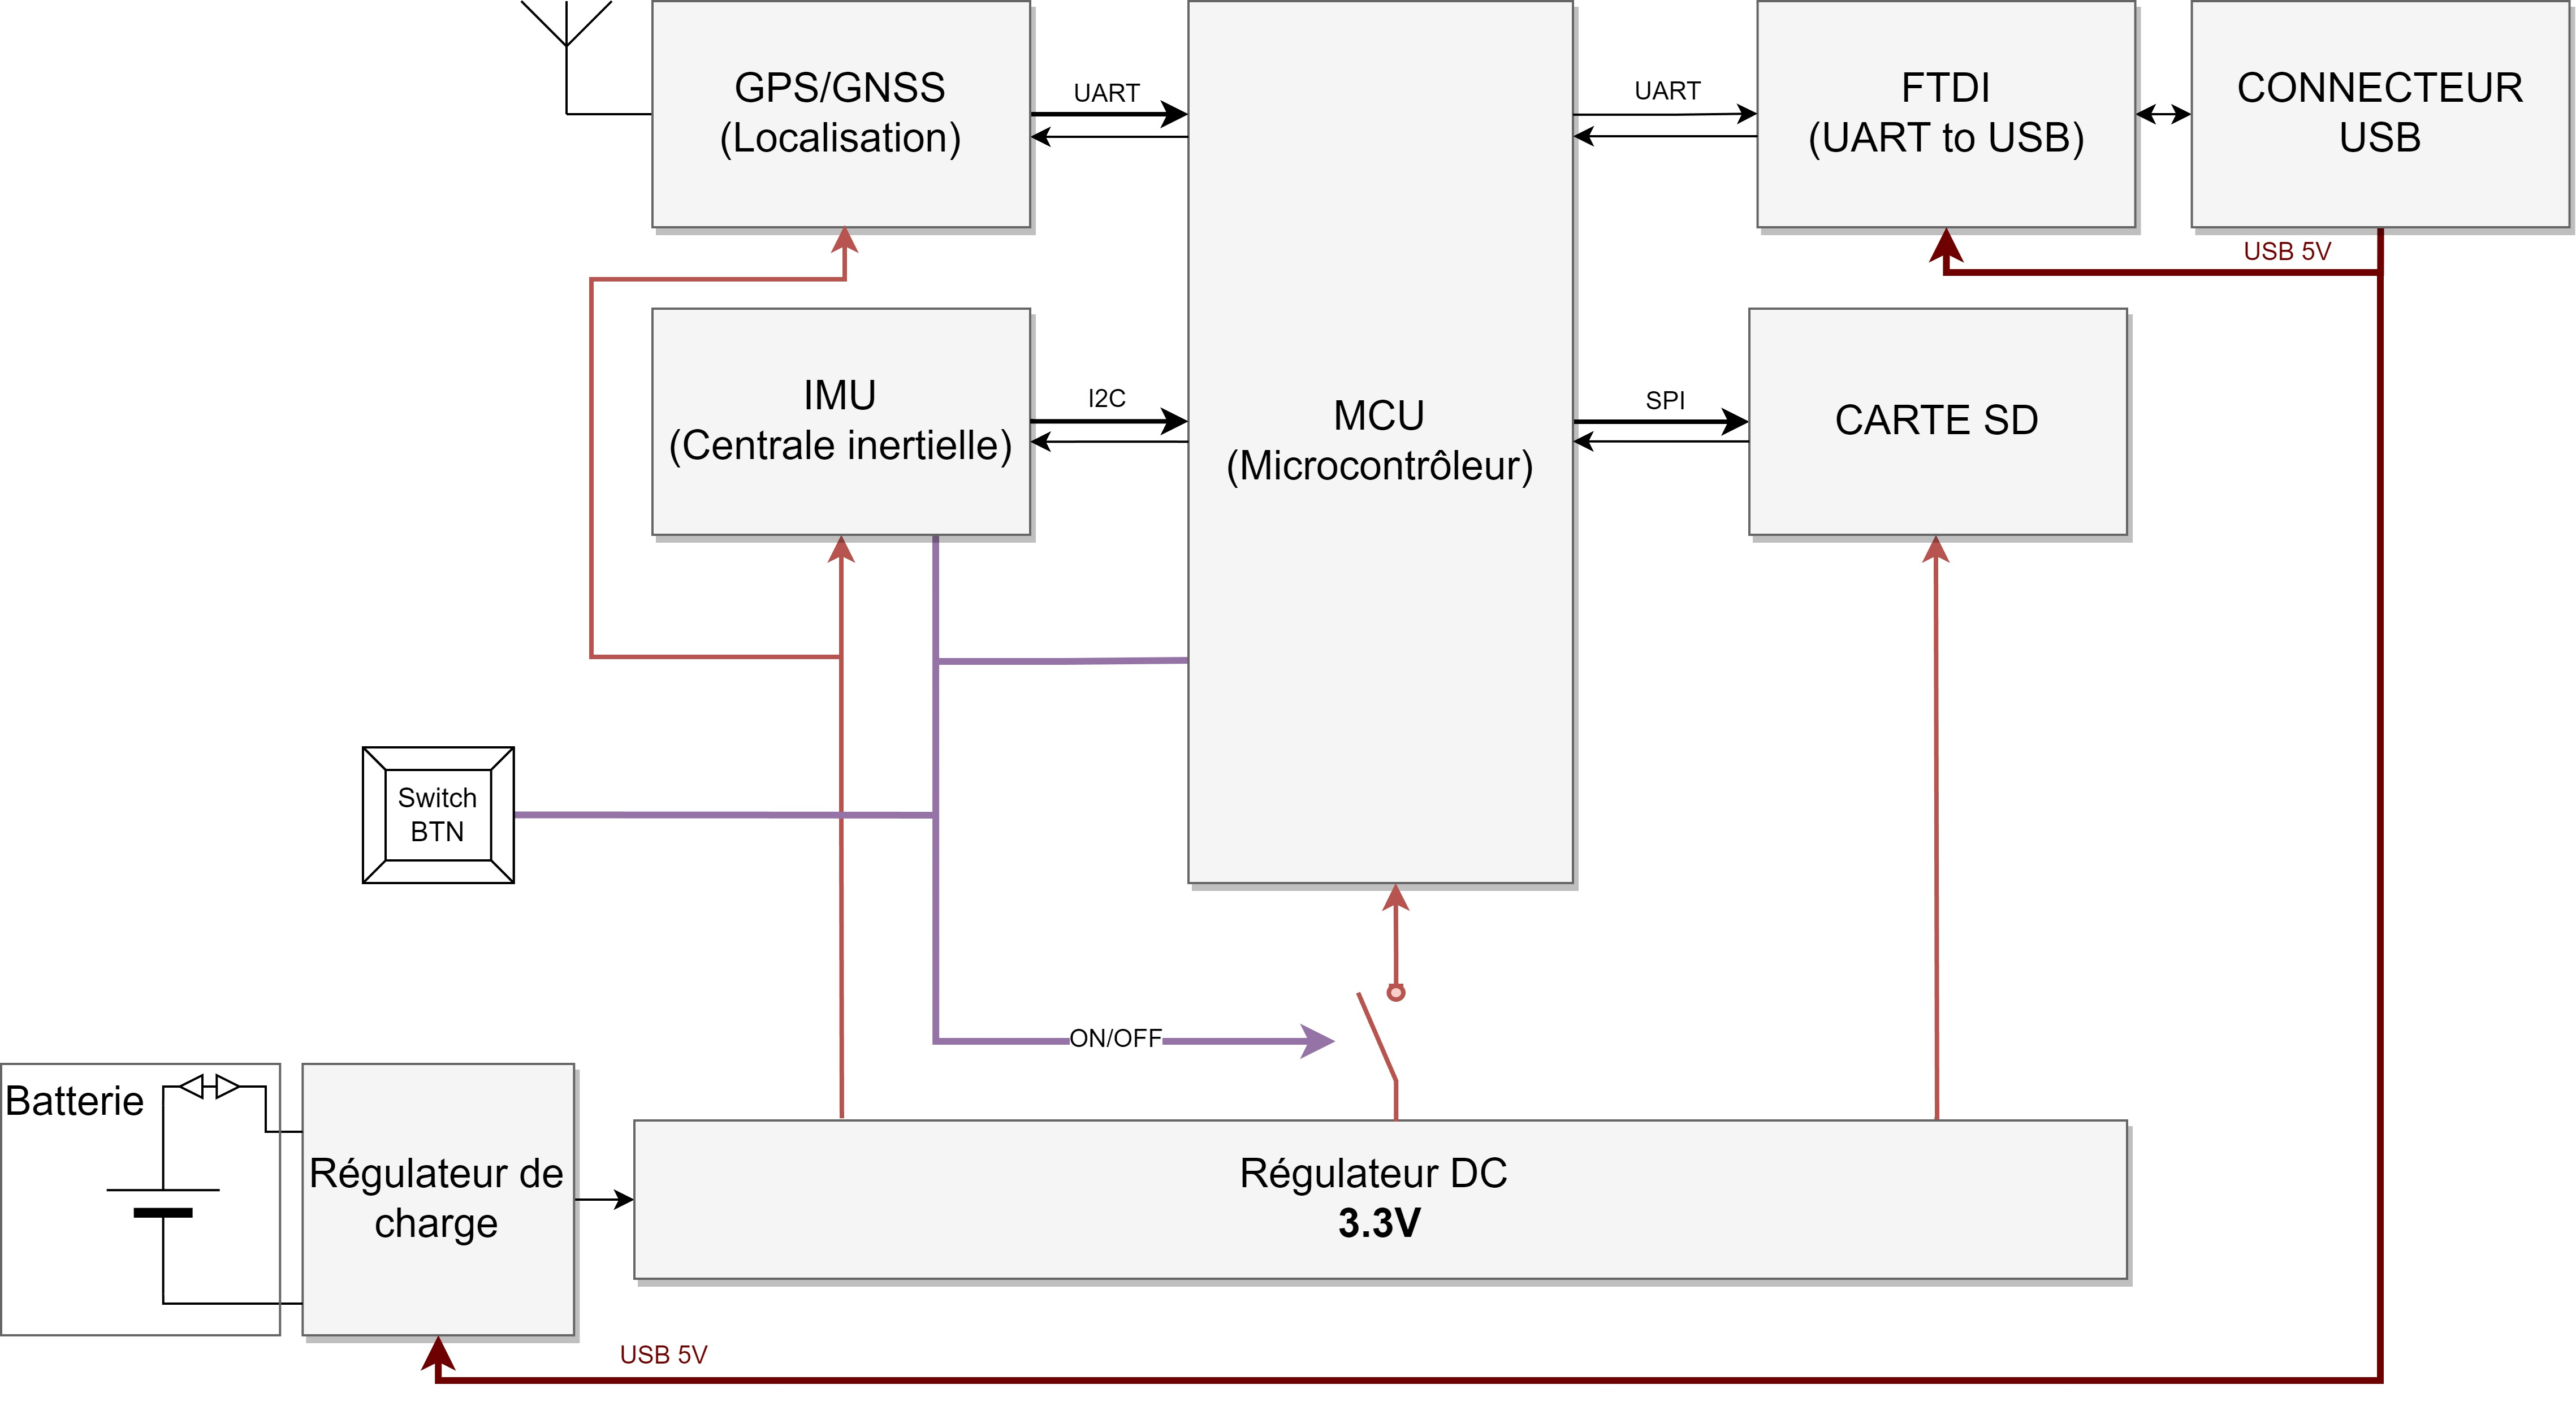
\includegraphics[width=1\textwidth]{../figures/cdc/blocs_grossiers_no_antenna.jpg}
	\caption{Schéma bloc}
	\label{fig:schbloc}
	\source{Auteur}
\end{figure}
% ---- Description des blocs ----
\subsection{Description des blocs} \label{ssec:Desc-blocs}

\begin{table}[h]
	\resizebox{\columnwidth}{!}{%
		\begin{tabular}{|l|l|}
			\hline
			Bloc         & Description                                                                         \\ \hline
			\Gls{gnss}.  & Récepteur \Gls{rf} avec antenne interne/externe et communication UART.              \\ \hline
			\Gls{mcu}.   & Microcontrôleur PIC32, intelligence du système, basse consommation.                 \\ \hline
			\Gls{imu}.   & Centrale inertielle, accélération, gyroscope...                                     \\ \hline
			Carte SD     & Stockage des données de vol.                                                        \\ \hline
			\Gls{FTDI}.  & Convertis la communication USB en série.                                            \\ \hline
			Régulateurs. & Le régulateur de charge gère la charge de l'accu. et un régulateur 3.3V le suit.    \\ \hline
			Batterie.    & La batterie est un accu que l'on peut charger par USB et permet une bonne autonomie. \\ \hline
		\end{tabular}%
	}
\end{table}

\clearpage
\raggedbottom
\subsection{Choix des composants et technologies} \label{sssec:ComposantsTech}
L'objectif de la pré-étude consiste en grande partie à sélectionner méthodiquement les technologies et les composants du projet. Cette partie du travail est essentielle et critique.

\subsubsection{Microcontrôleur}
Le microcontrôleur nécessite au minimum les périphériques suivants : \\
\fbox{2 UART} \fbox{1 SPI} \fbox{1 I2C} \\
Il est préférable que le \gls{mcu} dispose de différentes configurations de gestion de puissance, notamment des modes d'économie d'énergie, afin d'avoir une maîtrise de la consommation et de permettre une meilleure autonomie. Enfin, le standard de l'école veut que les familles de microcontrôleurs PIC32 (Microchip) sont préférées.

\begin{figure}[h]
	\centering
	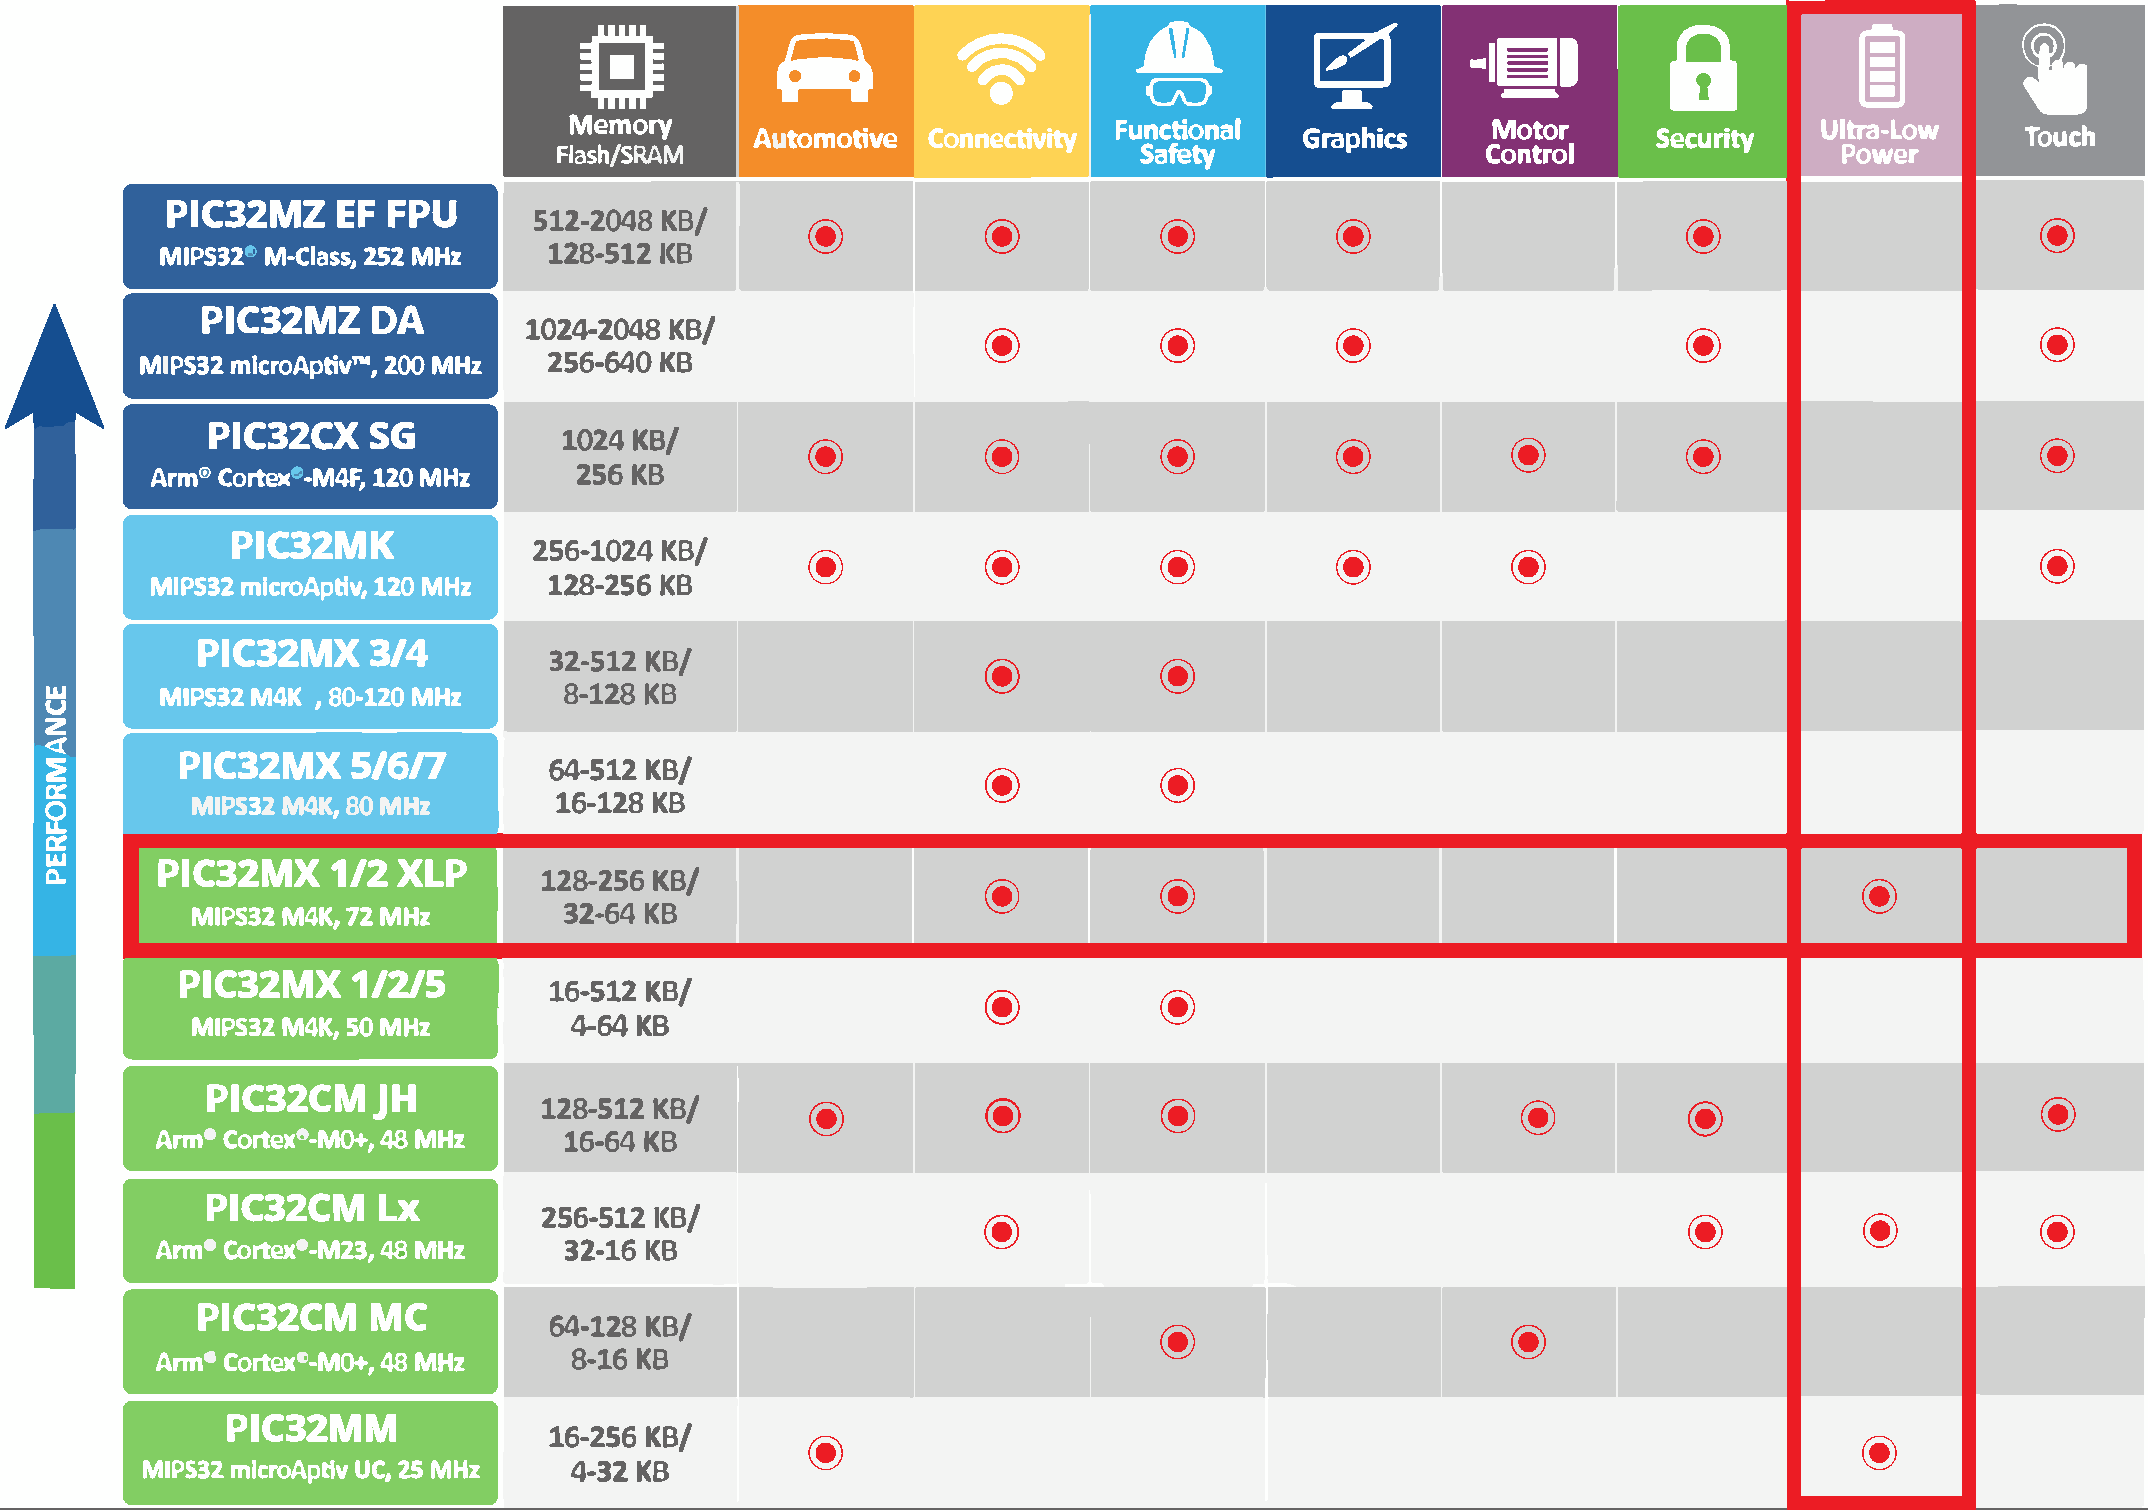
\includegraphics[width=0.65\linewidth]{../figures/pre_etude/familles_pic32}
	\caption{Familles PIC32}
	\label{fig:famillespic32}
	\source{\href{https://www.microchip.com/en-us/products/microcontrollers-and-microprocessors/32-bit-mcus/pic32-32-bit-mcus}{Microchip, familles}}
\end{figure}

Sur la figure \ref{fig:famillespic32} le \gls{mcu} sélectionné appartient à la gamme MX (Baseline performance-mémoire) et à la famille XLP qui offre notamment la fonctionnalité "Ultra low power" qui est celle qui nous intéresse.

\begin{figure}[h]
	\centering
	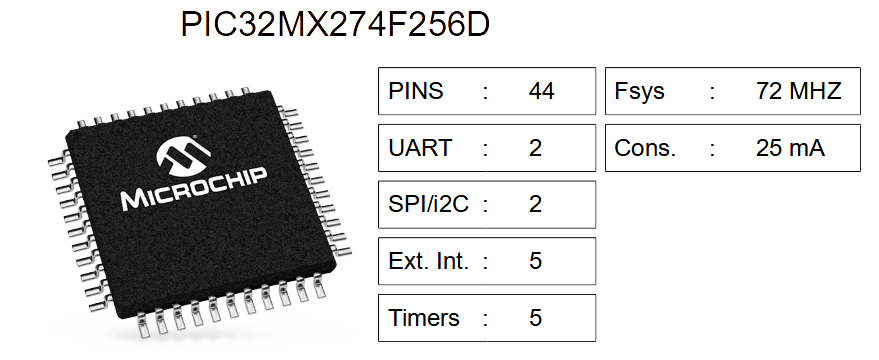
\includegraphics[width=0.7\linewidth]{../figures/pre_etude/Carac_PIC32}
	\caption{Caractéristiques du PIC32 choisi}
	\source{Auteur}
	\label{fig:caracpic32}
\end{figure}

\clearpage
\subsubsection{Centrale inertielle} 
Pour la centrale inertielle, il existe un composant avec lequel j'ai déjà acquis une certaine expérience et eu l'occasion d'utiliser et de créer des librairies pour le firmware en C. Celui-ci est performant et très utilisé dans l'industrie. Il est hautement configurable et a le grand avantage de calculer déjà une fusion de capteurs ainsi qu'une compensation de la dérive par les mesures de température. Cela permet notamment d'accéder à des données plus poussées, telles que les quaternions et les angles d'Euler. Il s'agit du \fbox{\href{https://www.bosch-sensortec.com/products/smart-sensors/bno055/}{BNO055}} de BOSCH.
 
\begin{center}
	\underline{Caractéristiques importantes :} \\
	\begin{tabular}{l l l l}
		Résolution gyroscope & : & 16 & [bits] \\
		Résolution accéléromètre & : & 14 & [bits] \\
		Résolution magnétomètre & : & $\sim$0.3 & [$\mu$T] \\
		$I_{DD}$ & : & 12.3 & [mA] \\
		Dérive de température & : & $\pm$ 0.03 & [\%/K] \\ 
		Dérive accéléromètre & : & 0.2 & [\%/V] \\
		Dérive gyroscope & : & <0.4 & [\%/V]
	\end{tabular} \\
\end{center}

Afin de simplifier l'implémentation de ce composant dans le projet, sachant qu'il s'agit d'un boîtier \textit{28-TFLGA} difficile à souder ou à mettre au four, il est possible d'utiliser la carte miniature d'Adafruit, cette carte comprend tous les composants passifs requis. Cela facilite ainsi son montage sur le \gls{pcb}.

\begin{figure}[h]
	\centering
	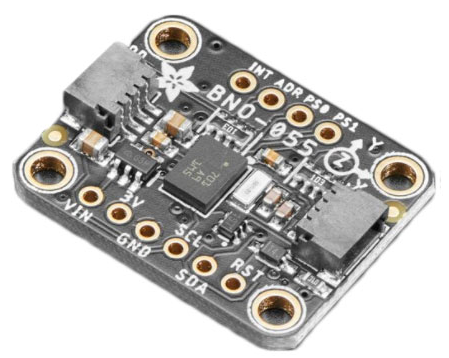
\includegraphics[width=0.4\linewidth]{../figures/pre_etude/BNO055_Adafruit}
	\caption{Carte d'extension, centrale inertielle}
	\source{\href{https://www.digikey.ch/en/products/detail/adafruit-industries-llc/4646/12609996?s=N4IgTCBcDaIEYDsD2AGArGgBAQwCbYDMAnAVwEsAXEAXQF8g}{Digikey, 4646}}
	\label{fig:bno055adafruit}
\end{figure}

\begin{center}
	\underline{Données disponibles :}
	\begin{table}[h]
		\centering
		\begin{tabular}{|ll|}
		\hline
		Température & \\
		\hline
		Vecteur gravité & XYZ \\
		\hline
		Orientation compensées, quaternion & WXYZ \\
		\hline
		Orientation compensée, angle de Euler & HPR \\
		\hline
		Données gyroscopiques & XYZ \\
		\hline
		 Intensité du champ magnétique & XYZ \\
		\hline
		Accélération & XYZ \\
		\hline
	\end{tabular}
	\caption{Liste des données accessibles}
	\end{table}
\end{center}

\clearpage

\subsubsection{GPS / GNSS}
Pour le \gls{GPS}/\gls{GNSS}, différents critères entrent en jeu dans le cadre de ce projet : le prix, la facilité d'implémentation, la complexité (par complexité, nous entendons le nombre de fonctionnalités), la consommation et la performance.

Il existe un très grand nombre de récepteurs \gls{rf} pour la navigation. Parmi les plus utilisés dans l'industrie, dont l'implémentation est la plus simple et la documentation la plus complète, il y a plusieurs gammes chez le fabricant \fbox{ublox}.
Deux composants ont principalement été pris en considération :
Le \textbf{CAM-M8C-0} (BeiDou, GLONASS, GNSS, GPS, QZSS) avec une antenne omnidirectionnelle interne au composant et différents modes de puissance, ainsi que le \textbf{MAX-M10M-00B} (BeiDou, Galileo, GLONASS, GNSS, GPS) sans antenne interne mais avec une consommation de base plus faible.

\begin{figure}[h]
	\centering
	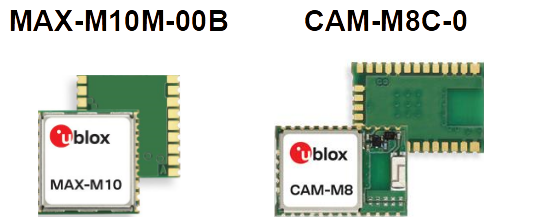
\includegraphics[width=0.6\linewidth]{../figures/pre_etude/img_gnss}
	\caption{Illustration des deux GNSS}
	\source{\href{https://www.digikey.ch/fr/products/detail/u-blox/CAM-M8C-0/6150647?s=N4IgTCBcDaIMIEECyBaJAOOKAMIC6AvkA}{Digikey, MAX-M10 et CAM-M8C}}
	\label{fig:imggnss}
\end{figure}


\begin{figure}[h]
	\centering
	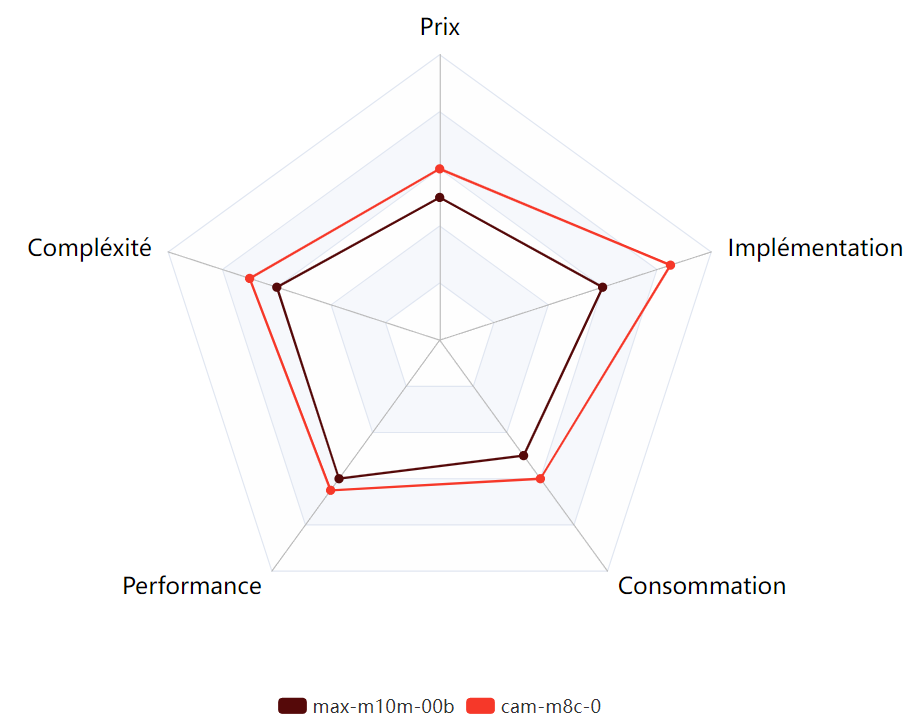
\includegraphics[width=0.65\linewidth]{../figures/pre_etude/Comp_GNSS}
	\caption{Comparaison GNSS}
	\source{Auteur}
	\label{fig:compgnss}
\end{figure}

Malgré les différents avantages que présente le MAX-M10M-00B sur la figure \ref{fig:compgnss}, le choix s'est porté sur CAM-M8C-0 grâce à sa facilitée d'implémentation et à la garantie du fabricant sur son antenne omnidirectionnelle de qualité.

\clearpage

\subsubsection{Carte SD} 
Les pilotes de carte SD disponibles dans \gls{harmony} ne permettent pas une gestion des capacités de stockage trop importantes. Cela signifie, que nous ne pouvons pas avoir des cartes SD de trop grandes capacités, c'est pour cela que nous allons baser nos dimensionnements sur une carte de \textbf{256MB}. 

\begin{figure}[h]
	\centering
	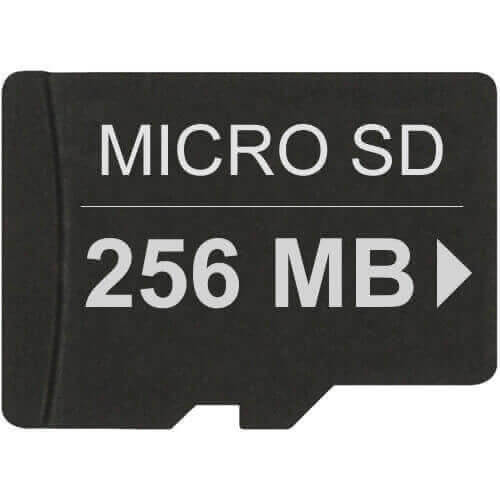
\includegraphics[width=0.2\linewidth]{../figures/pre_etude/CarteSD_Illustration}
	\caption{Illustration carte SD}
	\source{\href{https://www.oempcworld.com/OEMPCworld-com/017045.html}{https://www.oempcworld.com/OEMPCworld-com/017045.html}}
	\label{fig:cartesdillustration}
\end{figure}


\paragraph{Estimation de la capacité} Admettons les paramètres suivants où $S$ représente une taille de données et $T$ un temps :

\begin{tabular}{lrl}
	$S_{SD}$ & $256$ & $[KB]$ \\
	$S_{gyro}$ & $16$ & $[Bytes]$ \\
	$S_{accel}$ & $16$ & $[Bytes]$ \\
	$S_{gnss}$ & $\sim100$ & $[Bytes]$ \\
	$T_{inertiel}$ & $0.5$ & $[s]$ \\
	$T_{gnss}$ & $5$ & $[s]$ \\
	$T_{mesMin}$ & $900$ & $[s]$ \\
\end{tabular}

Nous pouvons déduire la taille mémoire que prendra 5 secondes d'enregistrement avec les paramètres par défaut du système : 
\begin{equation*}
	S_{single} = \frac{T_{gnss}}{T_{inertiel}}(S_{gyro}+S_{accel}) + S_{gnss} = \frac{5}{0.5}(16+16) + 100 = 420 \; [Bytes]
\end{equation*}

Nous pouvons enfin calculer à partir de cela, la taille mémoire que prendra 15 minutes d'enregistrement : 

\begin{equation*}
	S_{mesures} = \frac{S_{single}}{T_{gnss}} * T_{mesMin} = \frac{420}{5} * 900 = 75'600 \; [Bytes] = 75.6 \; [KB]
\end{equation*}

Nous pouvons déduire avec cette estimation qu'une carte SD de 256MB est largement suffisante et permet de mesurer jusqu'à un temps calculable de cette façon :

\begin{equation*}
	T_{mesures} = \frac{S_{SD}*T_{gnss}}{S_{single}} = \frac{256'000*5}{420} = \sim508 \; Minutes = \sim8.5 \; Heures
\end{equation*}

Nous estimons donc, que les données de vol des 8.5 dernières heures sont enregistrées dans la carte SD.

\clearpage

\subsection{Batterie, autonomie, charge et régulation} 
Afin de dimensionner une batterie pour le projet, il faut considérer les différentes consommation :

\begin{center}
	\underline{Liste des consommations principales} \\
	\begin{table}[h]
		\centering
		\begin{tabular}{lrll}
			Microcontrôleur & 24 & [mA] & Typ. \\
			Carte-SD & ~100 & [mA] & Max. \\
			Carte-SD & ~60 & [mA] & Moyenne \\
			\gls{imu} & 12.3 & [mA] & Typ. \\
			\gls{GNSS} & 71 & [mA] & Max. \\
			\gls{GNSS} & 29 & [mA] & Typ. \\
			\hline
			Totale max & \underline{207.3} & [mA] & Max. \\
			Totale moyennes & \underline{125.3} & [mA] & Moyenne \\
			\hline
		\end{tabular}
		\caption{Tableau des consommations de courant}
		\label{tab:consommateur}
	\end{table}
\end{center}

En examinant les consommations typiques et moyennes du tableau \ref{tab:consommateur} à régime constant, et en visant une autonomie de \fbox{\textbf{10 heures}}, nous aurions besoin d'une batterie d'une capacité de \fbox{\textbf{1253 mAh}}.

\paragraph{Technologies} Concernant la technologie de la batterie, notre objectif, dans un souci d'ergonomie, est de permettre son chargement via un connecteur USB. La technologie offrant actuellement la meilleure densité d'énergie est le \fbox{Lithium Ion}\footnote{\href{https://www.epectec.com/batteries/cell-comparison.html}{https://www.epectec.com/batteries/cell-comparison.html}}. Elle présente cependant des inconvénients, énumérés dans le tableau \ref{tab:inconvlion}.

\begin{table}[h]
	\centering
	\begin{tabular}{l|l}
		Avantages &  Inconvénient\\
		\hline
		Haute densité d'énergie. & Risque d'éclatement. \\
		Poids léger. & Risque d'enflammement avec l'eau. \\ 
		Haute durée de vie. & Sensible a la température. \\
		Charge rapide. & Décharge complète altérante. \\
		\hline
	\end{tabular}
		\caption{Tableau avantages/inconvénient LI-ION}
		\label{tab:inconvlion}
\end{table}

Les inconvénients listés dans le tableau \ref{tab:inconvlion} posent un risque pour l'intégrité des données de la carte-SD. C'est pourquoi il est essentiel de bien dimensionner le boîtier ainsi que l'intégration du circuit et de la batterie pour pallier ces dangers. Malgré les risques du Li-Ion, il s'agit d'une technologie très utilisée, y compris dans des domaines sensibles.

\clearpage

\paragraph{Choix de la batterie} La batterie doit avoir une capacité d'au moins \textbf{1260 mAh} et être suffisamment compacte pour être intégrée dans un boîtier de petite taille. Une batterie répond à ces critères : il s'agit de la \fbox{\textbf{PICPAL36}} de chez Farnell\footnote{Distributeur de composants électroniques. \href{https://ch.farnell.com/en-CH/panasonic/picpal36/battery-li-ion-1-3ah-3-7v/dp/2819223}{Lien de la batterie.}}. Les dimensions et caractéristiques de cette batterie sont visibles sur les figures \ref{fig:batt} et \ref{fig:caracbatt}.

\begin{figure}[h]
	\centering
	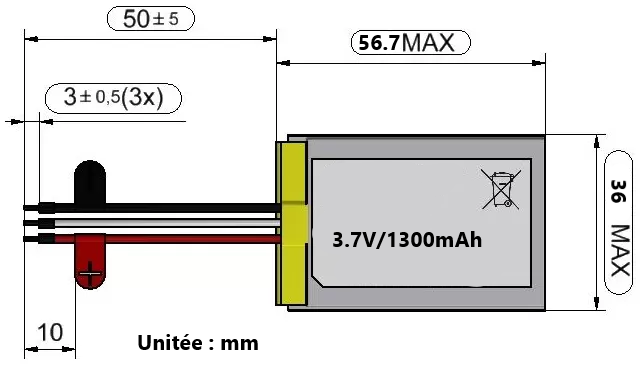
\includegraphics[width=0.55\linewidth]{../figures/pre_etude/batt}
	\caption{Dimension de la batterie}
	\label{fig:batt}
	\source{Auteur}
\end{figure}

\begin{figure}[h]
	\centering
	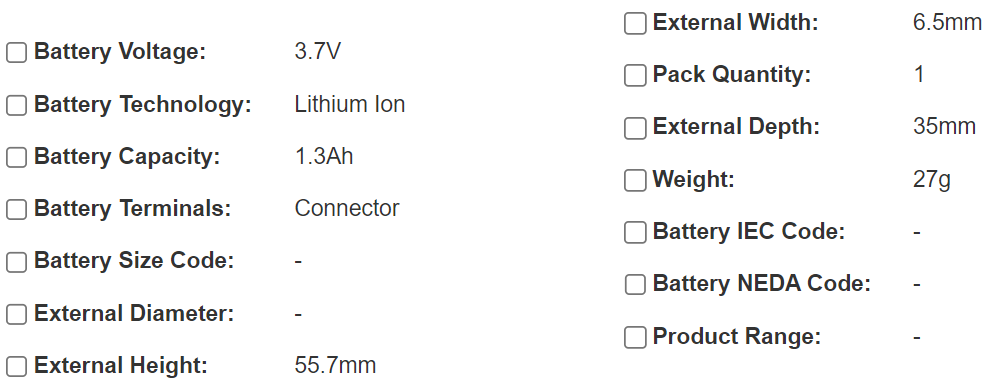
\includegraphics[width=0.7\linewidth]{../figures/pre_etude/Carac_Batt}
	\caption{Caractéristiques de la batterie}
	\label{fig:caracbatt}
\end{figure}

\paragraph{Régulateur de charge} Le choix du régulateur de charge s'est orienté vers un composant déjà utilisé par l'école, dont les caractéristiques et le montage sont bien connus. C'est un composant performant et fréquemment employé. De plus, il est disponible dans le stock de composants de l'école. Il s'agit du \fbox{\textbf{MCP73871T-2CCI/ML}}. Il est configurable et permet la charge des batteries Li-ion et Li-po.

\begin{figure}[h]
	\centering
	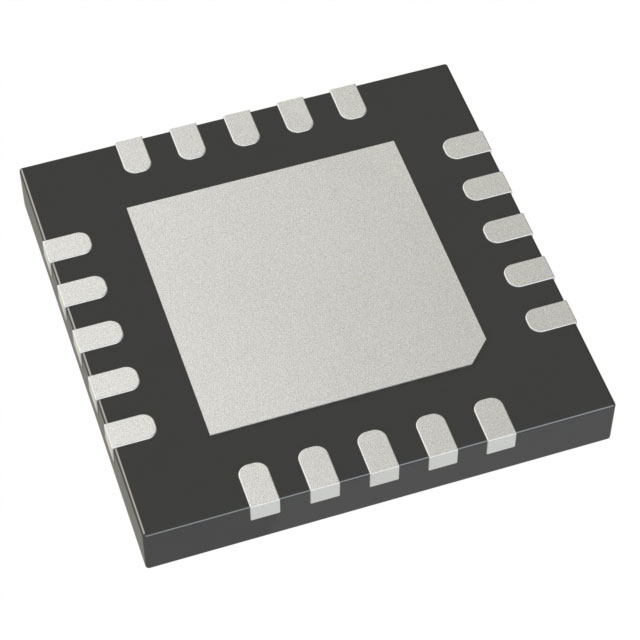
\includegraphics[width=0.2\linewidth]{../figures/pre_etude/MCP}
	\caption{MCP73871T-2CCI/ML}
	\source{\href{https://www.digikey.ch/fr/products/detail/microchip-technology/MCP73871T-2CCI-ML/7065594}{Digikey IC BATT CHG LI-ION 1CELL 20QFN}}
	\label{fig:mcp}
\end{figure}


\clearpage

\subsection{Systèmes d'économie d'énergies} 

Au-delà des 10 heures d'autonomie estimées, il est envisageable, pour maximiser le temps de logging, d'adopter des mécanismes d'économie d'énergie. Ces mécanismes pourraient être :

\paragraph{$\bullet$ Modes de puissance du PIC32} Le microcontrôleur peut basculer entre différents modes de puissance où il réduit à la fois sa consommation et ses fonctionnalités. On pourrait envisager de passer en mode d'énergie restreinte entre les périodes d'enregistrement ou de limiter l'utilisation de certains périphériques.

\paragraph{$\bullet$ Modes de puissance du \gls{GNSS}} À l'instar du \gls{mcu}, le composant de navigation dispose de plusieurs modes de fonctionnement qui permettent d'économiser de l'énergie. Un mode particulièrement utile permet de limiter sa cadence de données à 1Hz, étant donné qu'il n'est pas nécessaire qu'il fournisse des informations de localisation aussi fréquemment.

\paragraph{$\bullet$ Alimentation du \gls{GNSS}} On pourrait également envisager de ne pas alimenter le \gls{GNSS} lorsqu'il n'est pas en service, afin de supprimer complètement sa consommation entre chaque mesure.

\paragraph{$\bullet$ Modes de puissance \gls{imu}} La centrale inertielle dispose également de différents modes. Ces modes permettent, par exemple, de limiter les mesures à certains axes ou de la mettre en veille. Elle se met d'ailleurs automatiquement en veille après un certain temps entre les mesures. Ces modes peuvent être utilisés efficacement.

\paragraph{$\circ$ Alimentation de la carte SD} Il est envisageable d'éteindre entièrement la carte SD entre les écritures. Cependant, étant donné que les écritures seront fréquentes, l'intérêt de cette démarche est limité.

\paragraph{$\bullet$ Mise en veille automatique du système} Si aucun mouvement n'est détecté après un certain délai, il est envisageable que le système s'éteigne entièrement.

\subsection{Diagramme des états du système} 

\begin{figure}[h]
	\centering
	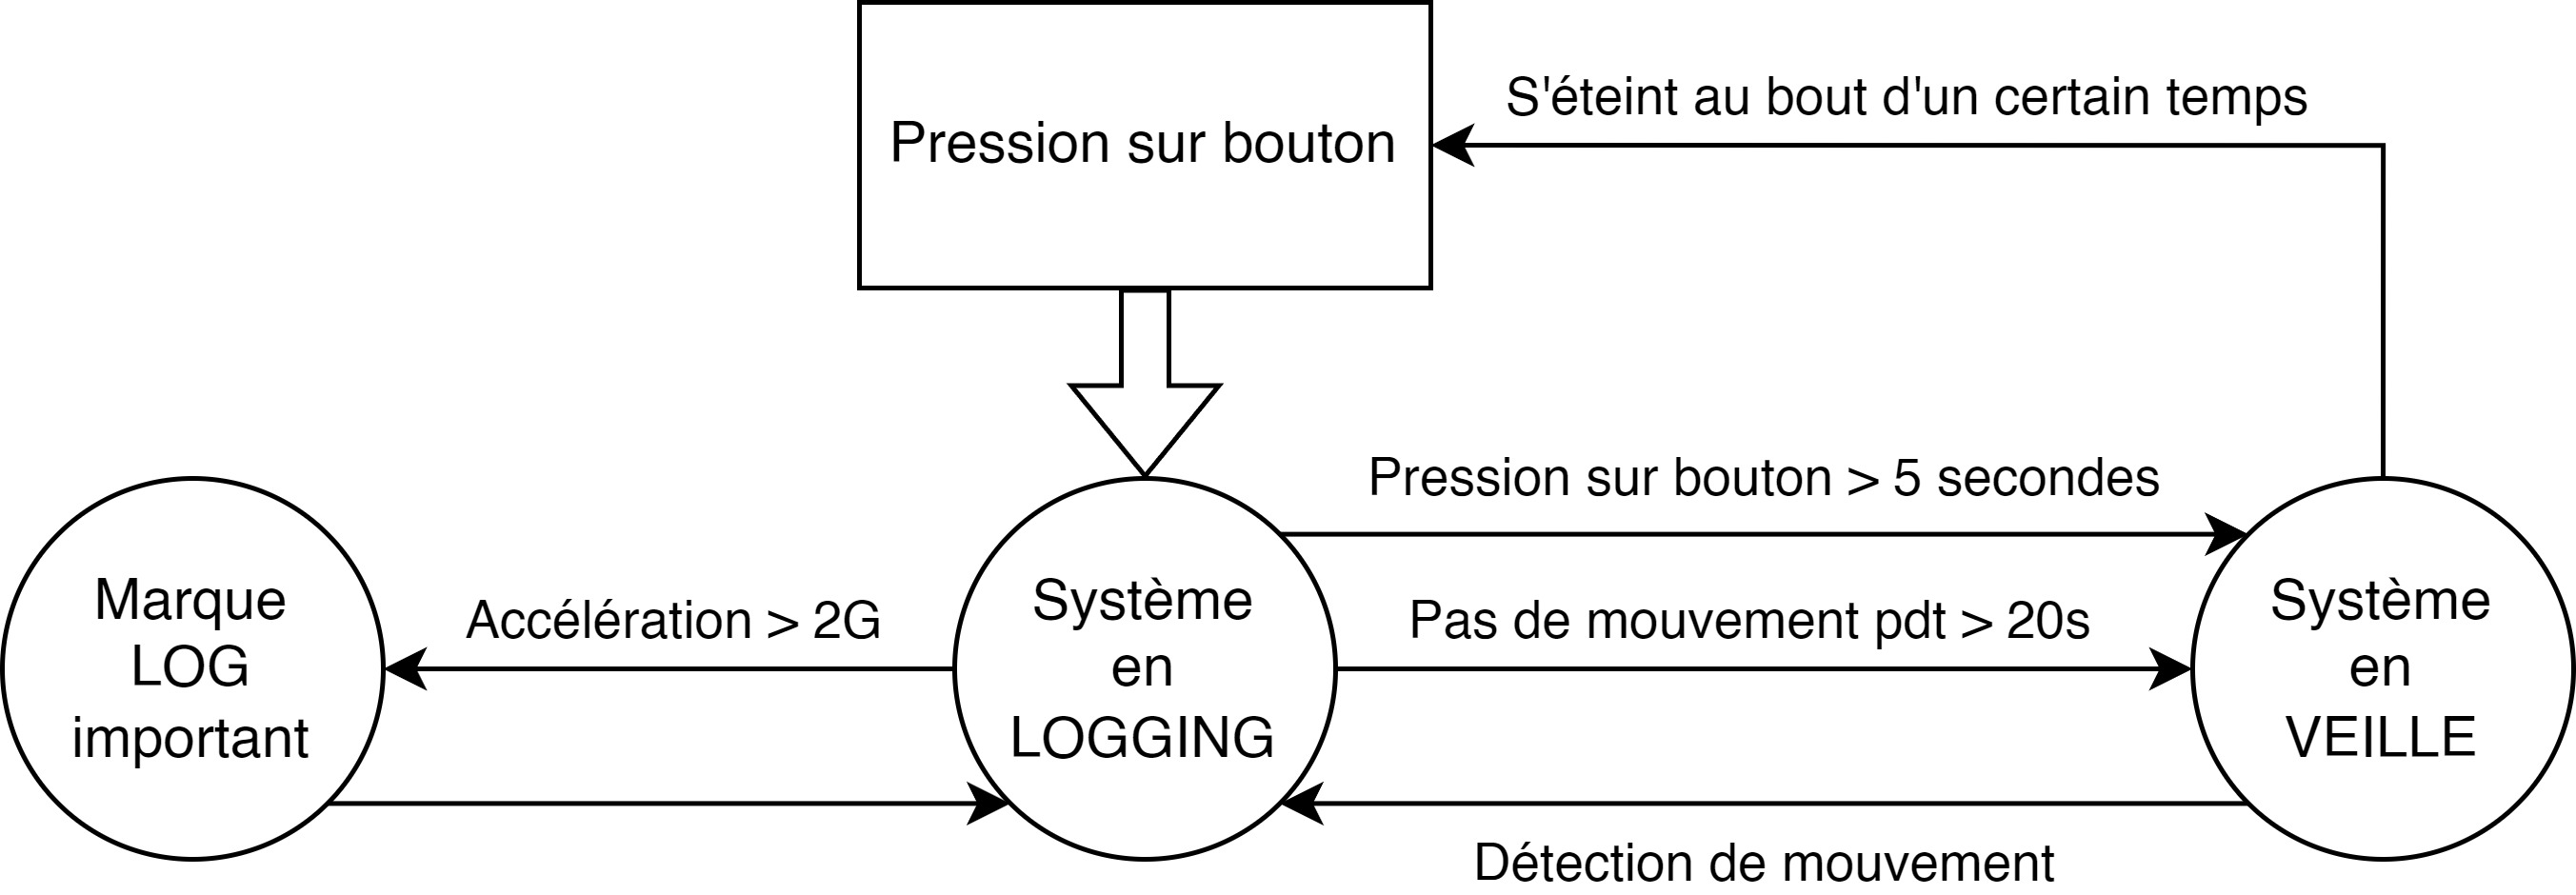
\includegraphics[width=0.8\linewidth]{../figures/pre_etude/Diagramme_Etat_Preetude}
	\caption{Diagrammes des états (Sans USB)}
	\source{Auteur}
	\label{fig:diagrammeetatpreetude}
\end{figure}

Sur la figure \ref{fig:diagrammeetatpreetude} les états de communication par le port USB ne sont pas représentés, il s'agit des modes principaux.


\clearpage

\subsection{Estimation des coûts} \label{ssec:Estimation-Couts}

À partir des composants et des technologies définis lors de la pré-étude, nous pouvons estimer le coût du projet. Cette estimation est présentée dans le tableau \ref{tab:estimcouts}.

\begin{center}
	\underline{Estimation des coût} 
	\vspace{-4mm}
	\begin{table}[h]
		\centering
		\begin{tabular}{lr}
			Élément & Prix estimé \\
			\hline
			\gls{pcb} & 60.- \\
			Batterie & 36.- \\
			\gls{imu} & 26.- \\
			\gls{GNSS} & 24.- \\
			Boîtier & 20.- \\
			Composants divers & 15.- \\
			\gls{mcu} & 6.- \\
			Régulateurs & 6.- \\
			USB \& \gls{FTDI} & 3.- \\
			\hline
			Total & \underline{196.-} \\
			\hline
		\end{tabular}
		\caption{}
		\label{tab:estimcouts}
	\end{table}
\end{center} \vspace{-5mm}

Cette estimation est relativement élevée. Il est à noter que le coût du \gls{pcb} pourrait être réduit en cas de commande groupée dans un panel\footnote{Regroupement de plusieurs circuits imprimés en un seul, pour diminuer le coût.}. Par ailleurs, les prix du boîtier et des composants semblent également être assez élevés.


\subsection{Conclusion et perspectives de la Pré-étude}

\textbf{Fonctionnement du système:}
La conception du système semble possible, le microcontrôleur s'interface avec quatre périphériques essentiels : un \gls{GNSS} pour la localisation, une centrale inertielle pour des mesures sur 9 axes (priorisant les mesures gyroscopiques et d'accélération), une carte SD pour le stockage (conservant au moins 15 minutes de données de vol), et un périphérique \gls{FTDI} pour l'interface avec un ordinateur via USB-C.

\textbf{Choix des composants et technologies:}
\begin{itemize}
	\item \textit{Microcontrôleur}: Requiert au moins 2 UART, 1 SPI, et 1 I2C. Le PIC32MX274F256D est privilégié car il offre divers modes d'économie d'énergie.
	\item \textit{Centrale inertielle}: Le BNO055 de BOSCH a été choisi, car il offre une variété de mesures avancées et une facilité d'implémentation grâce à la carte Adafruit.
	\item \textit{GPS/GNSS}: Le CAM-M8C-0 d'ublox a été retenu pour sa facilité d'implémentation et son antenne interne omnidirectionnelle.
	\item \textit{Carte SD}: Une capacité de 256MB a été choisie à cause des limites du pilote. Une telle carte permettrait d'enregistrer jusqu'à 8,5 heures de données de vol.
	\item \textit{Batterie, charge, et régulation}: Une capacité de 1253 mAh est nécessaire pour atteindre l'autonomie souhaitée de 10 heures. Une batterie compact de 1300 mAh a été retenue.
\end{itemize}

\textbf{Estimation des coûts:}
L'estimation totale pour le projet s'élève à environ 196 CHF. Néanmoins, il existe des possibilités d'économie, en particulier par une commande groupée du \gls{pcb}.

En conclusion, cette pré-étude a décortiqué le projet de façon méthodique pour sélectionner les composants et technologies appropriés. Elle a également fourni des estimations de coûts et identifié des mécanismes d'économie d'énergie potentiels. La prochaine étape consistera à entamer la phase de conception en utilisant ces informations utiles.
